%-------------------------
% Resume in Latex
% Author 1chooo
% License : MIT
%------------------------

%---- Required Packages and Functions ----

\documentclass[a4paper,11pt]{article}
\usepackage{latexsym}
\usepackage{xcolor}
\usepackage{float}
\usepackage{ragged2e}
\usepackage[empty]{fullpage}
\usepackage{wrapfig}
\usepackage{lipsum}
\usepackage{tabularx}
\usepackage{titlesec}
\usepackage{geometry}
\usepackage{marvosym}
\usepackage{verbatim}
\usepackage{enumitem}
\usepackage[hidelinks]{hyperref}
\usepackage{fancyhdr}
\usepackage{fontawesome5}
\usepackage{multicol}
\usepackage{graphicx}
\usepackage{cfr-lm}
\usepackage[T1]{fontenc}
\setlength{\multicolsep}{0pt} 
\pagestyle{fancy}
\fancyhf{} % clear all header and footer fields
\fancyfoot{}
\renewcommand{\headrulewidth}{0pt}
\renewcommand{\footrulewidth}{0pt}
\geometry{left=1.4cm, top=0.8cm, right=1.2cm, bottom=1cm}
% Adjust margins
%\addtolength{\oddsidemargin}{-0.5in}
%\addtolength{\evensidemargin}{-0.5in}
%\addtolength{\textwidth}{1in}
\usepackage[most]{tcolorbox}
\tcbset{
	frame code={}
	center title,
	left=0pt,
	right=0pt,
	top=0pt,
	bottom=0pt,
	colback=gray!20,
	colframe=white,
	width=\dimexpr\textwidth\relax,
	enlarge left by=-2mm,
	boxsep=4pt,
	arc=0pt,outer arc=0pt,
}

\usepackage{enumitem}
\setlist[itemize]{label=-, leftmargin=0cm, itemsep=0cm, topsep=0cm}

\urlstyle{same}

\raggedright
\setlength{\tabcolsep}{0in}

% Sections formatting
\titleformat{\section}{
  \vspace{-4pt}\scshape\raggedright\large
}{}{0em}{}[\color{olive}\titlerule \vspace{-7pt}]

%-------------------------
% Custom commands
\newcommand{\resumeItem}[2]{
  \item{
    \textbf{#1}{\hspace{0.5mm}#2 \vspace{-0.5mm}}
  }
}

\newcommand{\resumePOR}[3]{
\vspace{0.5mm}\item
    \begin{tabular*}{0.97\textwidth}[t]{l@{\extracolsep{\fill}}r}
        \textbf{#1}\hspace{0.3mm}#2 & \textit{\small{#3}} 
    \end{tabular*}
    \vspace{-2mm}
}

\newcommand{\resumeSubheading}[4]{
\vspace{0.5mm}\item
    \begin{tabular*}{0.98\textwidth}[t]{l@{\extracolsep{\fill}}r}
        \textbf{#1} & \textit{\footnotesize{#4}} \\
        \textit{\footnotesize{#3}} &  \footnotesize{#2}\\
    \end{tabular*}
    \vspace{-2.4mm}
}

\newcommand{\resumeProject}[4]{
\vspace{0.5mm}\item
    \begin{tabular*}{0.98\textwidth}[t]{l@{\extracolsep{\fill}}r}
        \textbf{#1} & \textit{\footnotesize{#3}} \\
        \footnotesize{\textit{#2}} & \footnotesize{#4}
    \end{tabular*}
    \vspace{-2.4mm}
}

\newcommand{\resumeSubItem}[2]{\resumeItem{#1}{#2}\vspace{-4pt}}

% \renewcommand{\labelitemii}{$\circ$}
\renewcommand{\labelitemi}{$\vcenter{\hbox{\tiny$\bullet$}}$}

\newcommand{\resumeSubHeadingListStart}{\begin{itemize}[leftmargin=*,labelsep=0mm]}
\newcommand{\resumeHeadingSkillStart}{\begin{itemize}[leftmargin=*,itemsep=1.7mm, rightmargin=2ex]}
\newcommand{\resumeItemListStart}{\begin{justify}\begin{itemize}[leftmargin=3ex, rightmargin=2ex, noitemsep,labelsep=1.2mm,itemsep=0mm]\small}

\newcommand{\resumeSubHeadingListEnd}{\end{itemize}\vspace{2mm}}
\newcommand{\resumeHeadingSkillEnd}{\end{itemize}\vspace{-2mm}}
\newcommand{\resumeItemListEnd}{\end{itemize}\end{justify}\vspace{-2mm}}
\newcommand{\cvsection}[1]{%
\vspace{2mm}
\begin{tcolorbox}
    \textbf{\large #1}
\end{tcolorbox}
    \vspace{-4mm}
}

\newcolumntype{L}{>{\raggedright\arraybackslash}X}%
\newcolumntype{R}{>{\raggedleft\arraybackslash}X}%
\newcolumntype{C}{>{\centering\arraybackslash}X}%
%---- End of Packages and Functions ------

%-------------------------------------------
%%%%%%  CV STARTS HERE  %%%%%%%%%%%
%%%%%% DEFINE ELEMENTS HERE %%%%%%%
\newcommand{\name}{Hugo ChunHo Lin} % Your Name
\newcommand{\course}{Dept. of Atmospheric Science, NCU.} % Your Program
\newcommand{\roll}{xxxxxxx} % Your Roll No.
\newcommand{\phone}{909-001068} % Your Phone Number
\newcommand{\emaila}{hugo970217@gmail.com} %Email 1
\newcommand{\emailb}{lcho0127@g.ncu.edu.tw} %Email 2
\newcommand{\myScore}{}
% \newcommand{\myScore}{GPA: 3.01/4.30; Rank: 25/33}


\begin{document}
\fontfamily{cmr}\selectfont
%----------HEADING-----------------


% \parbox{2.35cm}{%
% % 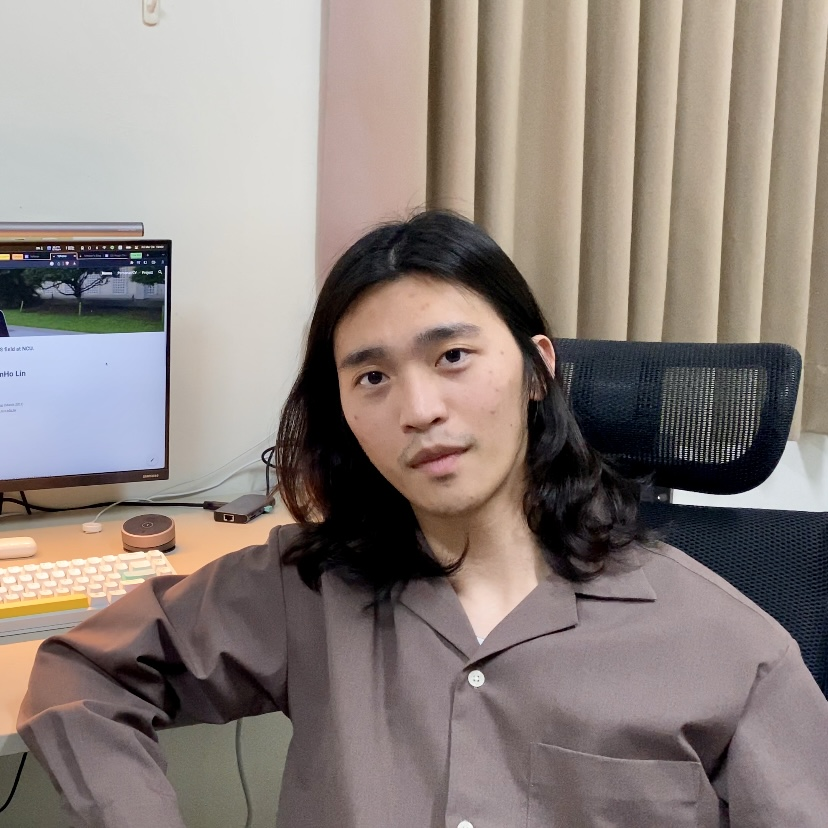
\includegraphics[width=2cm,clip]{IMG_4754.jpg}
% }
\parbox{\textwidth}{
\begin{tabularx}{\linewidth}{L r} \\
  \textbf{\huge \name} & {\raisebox{0.0\height}{\footnotesize \faPhone}\ +886-\phone}\\ The student who possesses a true passion for the CS field.
   & \href{mailto:\emaila}{\raisebox{0.0\height}{\footnotesize \faEnvelope}\ {\emaila}} \\
  XinYi, Taipei, Taiwan. & \href{https://1chooo-github-io.vercel.app/}{\raisebox{0.0\height}{\footnotesize \faGlobe}\ {1chooo's Portfolio}}\\
  {Major: \course} &  \href{https://github.com/1chooo}{\raisebox{0.0\height}{\footnotesize \faGithub}\ {1chooo (Hugo ChunHo Lin)}} \\
  {Minor Specialty: Dept. of CSIE, NCU.} & \href{https://www.linkedin.com/in/1chooo/}{\raisebox{0.0\height}{\footnotesize \faLinkedin}\ {Hugo ChunHo Lin}}
\end{tabularx}
}
% \parbox{3.0cm}{%
% \flushright 
\includegraphics[width=2cm,clip]{nitp_logo.png}
% }

\vspace{-3.0mm}

%-----------EDUCATION-----------------
\section{\textcolor{olive}{\textbf{Education}}}
  \resumeSubHeadingListStart
    \resumeSubheading
      { National Central University}{\myScore}
      {}{Sep. 2020 - present}
      % {Junior Student who possesses a true passion for the CS field.}{Sep. 2020 - present}
      \vspace{-5.0mm}
      \resumeItemListStart
        \item {\textbf{Major:} Dept. of Atmospheric Science; \textbf{Minor Specialty:} Dept. of CSIE}
        \item {\textbf{Course:} Alg, DS, Assembly, PPL, Degital Design, Weather and AI, etc.}
      \resumeItemListEnd      
  \resumeSubHeadingListEnd

\vspace{-6.5mm}

%-----------EXPERIENCE-----------------
\section{\textcolor{olive}{\textbf{Professional Experience}}}
  \resumeSubHeadingListStart
    \resumeSubheading
    { Amazon Web Services (AWS)}{}
    {Cloud Student Ambassador - Technical Support}{Aug. 2023 - present}

    \vspace{-2.0mm}
    \resumeItemListStart
        % \item {Workshops}
        % \item {Work description line 2}
    \resumeItemListEnd
    
    \vspace{-2.0mm}
    
    \resumeSubheading
    { Pegatron Corporation}{}
    {Software Engineer Summer Intern}{Jul. 2023 - Aug. 2023}
    \vspace{-2.0mm}
    
    \resumeItemListStart
        \item {\textbf{Smart Robot Smart World:} Prompt-based Learning for manipulating with the Visual-World Robot.}
        \item {By employing Prompt Engineering, I have increased support from 2 to 11 scenarios, a \textbf{450\%} improvement.}
        \item {The model accuracy has increased to \textbf{80\%} and now supports four objects, up from two.}
    \resumeItemListEnd
    
    \vspace{-2.0mm}
    
    \resumeSubheading
    { National Central University}{}
    {Teaching Assistant, Website Administrator}{}

    \vspace{-2.0mm}
    
    \resumeItemListStart
        \item {\textbf{Course:} Programmiing Python, Weather and Artificial Intelligence, Freshman English, Student Service-Learning.}
        \item {Launch a project aimed at developing a system to manage and track student progress.}
    \resumeItemListEnd
    
    % \vspace{-3.0mm}
      
  \resumeSubHeadingListEnd
  
\vspace{-6.5mm}

\section{\textcolor{olive}{\textbf{Extracurricular Activity}}}
  \resumeSubHeadingListStart
    \resumeSubheading
      { NCUFresh Team (NCUBlog)\hspace{0.5em} \href{https://github.com/ncufresh}{\faGithub} \hspace{0.2em} \href{https://22.ncufresh.ncu.edu.tw/blog/}{\faDesktop}} {}%Project Name
      {Website developer team for the incoming freshmen admitting to NCU.} %Project Name, Location Name
      {Dec. 2021 - Jul. 2022} %Event Dates

      \vspace{-2mm}
      
      \resumeItemListStart
        \item {The essential experience of manage larger projects with teammates.}
        \item {Frontend skills: UI/UX, Figma.}
        \item {Teamwork: leadership, meeting arrangement, facilitating communication, project demo.}
        \item {Marketing: increase social media reach, content of films and articles.}
      \resumeItemListEnd
    
    % \vspace{-3.0mm}
    
    
    \resumeSubheading
      { NCUApp Team (UI/UX \& Marketing)\hspace{0.5em} \href{https://github.com/NCUAppTeam}{\faGithub} \hspace{0.2em} \href{https://ncuappteam.github.io/}{\faDesktop}} {}%Project Name
      {The app developer team opens to all members of the NCU community.} %Project Name, Location Name
      {Mar. 2023 - present} %Event Dates

      \vspace{-2mm}

      \resumeItemListStart
        \item {The crucial experience managing existing projects with teammates to ensure that all functions are fully developed.}
        \item {Frontend skills: React Native, UI/UX, Figma.}
        \item {Marketing: product listings, map functionality, daily scheduling.}
      \resumeItemListEnd
    % \vspace{-3.0mm}
    
    
  %   \resumeSubheading
  %     { NCUAS Basketball Team (Co-captain)}{}
  %     {Basketball Team Co-captain in my department, Dept. ATM, NCU.}{Aug. 2022 - Jun. 2023}
  %     \vspace{-2.0mm}
  %     \resumeItemListStart
  %   % \item {Work description line 1}
  %   % \item {Work description line 2}
  %   \resumeItemListEnd
      
  % \resumeSubHeadingListEnd
      
  \resumeSubHeadingListEnd

\vspace{-6.5mm}

%-----------PROJECTS-----------------
\section{\textcolor{olive}{\textbf{Selected Projects}}}
    \resumeSubHeadingListStart
        \resumeProject
            { SIMPLE AI: Multi-User Machine Learning Education Platform \hspace{0.5em} \href{https://github.com/1chooo/simple-ai}{\faGithub} \hspace{0.2em} \href{https://www.youtube.com/watch?v=S0HZJIqVThI}{\faDesktop}} %Project Name
            {Develop a Line BOT utilizing \textbf{S3 and Amazon Recognition services} to enhance familiarity with NCU Campus.} %Project Name, Location Name
            {Aug. 2023} %Event Dates
        
            \vspace{-2mm}
        
            \resumeItemListStart
                \item {Training Model with Amazon Recognition and storing training data to AWS S3.}
                \item {Integrating with Line BOT using \textbf{Python Line Bot SDK and Flask}.}
                \item {Create an engaging storyline or narrative that enhances user interaction and exploration of the Central Campus.}
            \resumeItemListEnd
    
        % \vspace{-3mm}
    
        \resumeProject
            { BearBearYou: Campus Guide with AWS S3 and Recognition \hspace{0.5em} \href{https://github.com/1chooo/bear-bear}{\faGithub} \hspace{0.2em} \href{https://www.youtube.com/watch?v=S0HZJIqVThI}{\faDesktop}} %Project Name
            {Develop a Line BOT utilizing \textbf{S3 and Amazon Recognition services} to enhance familiarity with NCU Campus.} %Project Name, Location Name
            {Jun. 2022} %Event Dates
    
            \vspace{-2mm}
    
            \resumeItemListStart
                \item {Training Model with Amazon Recognition and storing training data to AWS S3.}
                \item {Integrating with Line BOT using \textbf{Python Line Bot SDK and Flask}.}
                \item {Create an engaging storyline or narrative that enhances user interaction and exploration of the Central Campus.}
            \resumeItemListEnd
        
        
        % \vspace{-3mm}
    
        \resumeProject
            { Evolving Beasts \hspace{0.5em} \href{https://github.com/1chooo/feather-feast}{\faGithub} \hspace{0.2em} \href{https://www.youtube.com/watch?v=S0HZJIqVThI}{\faDesktop}} %Project Name
            {Develop an online ordering system for leftovers using a real-time LINE BOT.} %Project Name, Location Name
            {Aug. 2023} %Event Dates
            
            \vspace{-2mm}
            
            \resumeItemListStart
                \item {Developed a Python Flask-based ordering system that integrates with various services, including providing functionalities for adding items and placing orders.}
                \item {What I have done: Developed a drama on LINE BOT and implemented databases using mySQL and servers. Created APIs to connect clients and the server using the Flask framework.}
            \resumeItemListEnd
            
        % \vspace{-3mm}
    
  \resumeSubHeadingListEnd
  
\vspace{-6.5mm}
  
%-----------Technical skills-----------------
\section{\textcolor{olive}{\textbf{Skills}}}

    \begin{itemize}[leftmargin=0.05in, label={}, itemsep=-2pt, topsep=0pt]
        \item \textbf{Programming Languages}: Python, c/c++, Java, Assembly, Go, JavaScripts, etc.
        \item \textbf{ML/DL}: Langchain, Keras, Tensorflow, Scikit-learn, Numpy, Pandas, etc.
        \item \textbf{DevOps}: AWS, Git, Docker, Bash, Linux, GitHub Action, mySQL, etc.
        \item \textbf{Languages}: English, Mandarin(Native).
    \end{itemize}

% \vspace{-4.0mm}
%-------------------------------------------
\end{document}
